\begin{figure}[!htbp]
\centering
\begin{subfigure}[b]{0.48\linewidth}
  \centering
  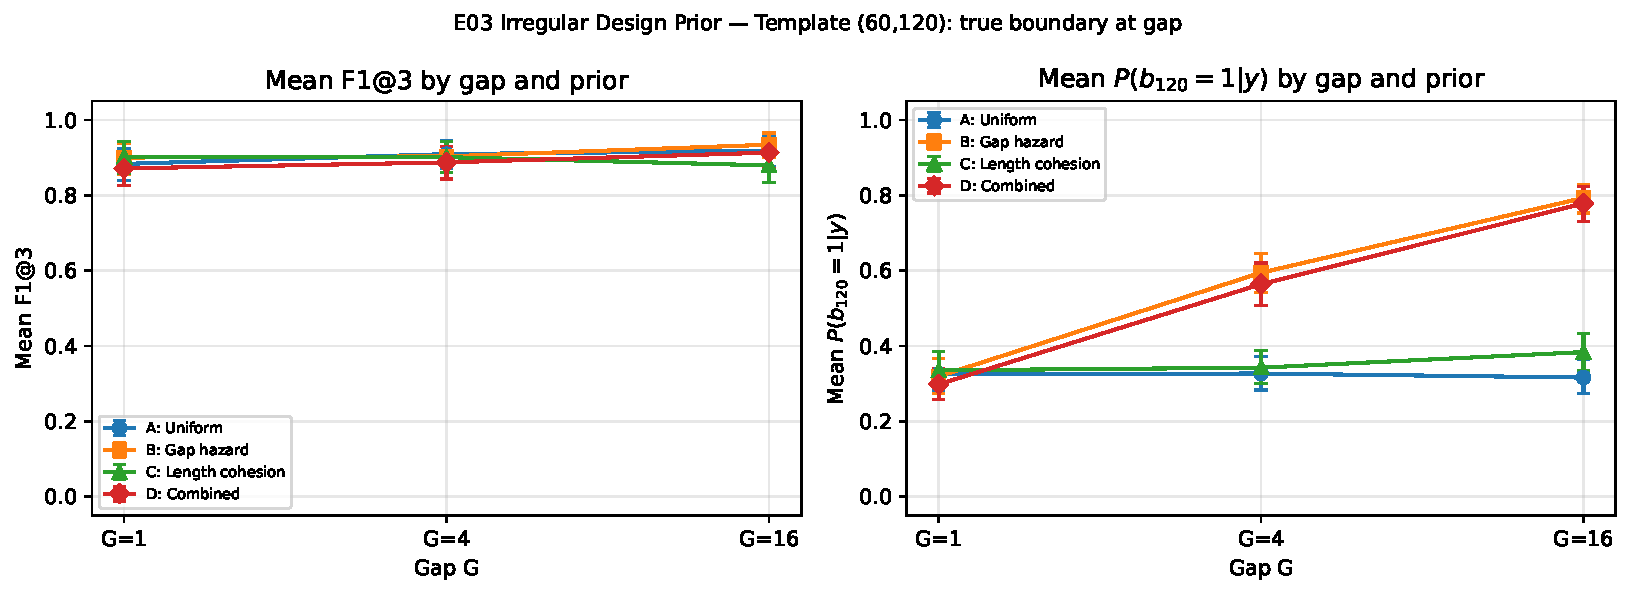
\includegraphics[width=\linewidth]{shared/figures/results/fig_E03_gap_true.pdf}
  \caption{True changepoint at position 120 (gap location). Posterior boundary probability
  at $i=120$ increases with gap size $G$ under priors B and D.}
  \label{fig:E03-gap-true-paper}
\end{subfigure}
\hfill
\begin{subfigure}[b]{0.48\linewidth}
  \centering
  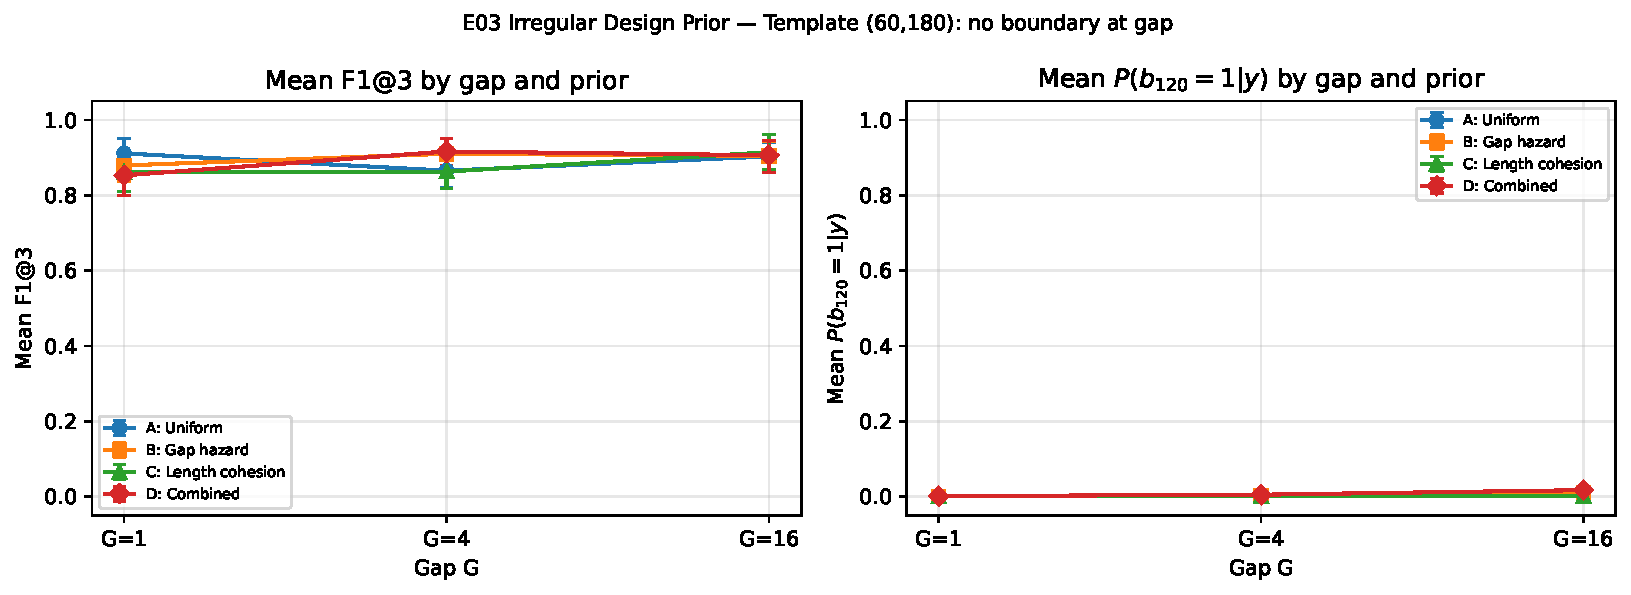
\includegraphics[width=\linewidth]{shared/figures/results/fig_E03_gap_false.pdf}
  \caption{No changepoint at position 120 (gap location). All priors assign near-zero
  posterior probability at the gap position regardless of gap size.}
  \label{fig:E03-gap-false-paper}
\end{subfigure}
\caption{E03 irregular-design prior ablation. Panels show mean boundary posterior $P(b_{120}=1\mid y)$
with 95\% bootstrap bands across 100 independent datasets. Left: template with true
changepoint at the large-gap position (60,\,120); right: template without a changepoint
at the gap (60,\,180). Gap hazard and combined priors (B, D) raise boundary probability
at the gap location when a true change is present, and remain near zero when it is absent.
All four priors preserve correct segmentation: mean F1@3 exceeds 0.85 in every cell.}
\label{fig:planned-irregular-paper}
\end{figure}
